\documentclass{standalone}
\usepackage{hsbcommon}
\usepackage{pgfplots}
\pgfplotsset{compat=1.18}
\begin{document}
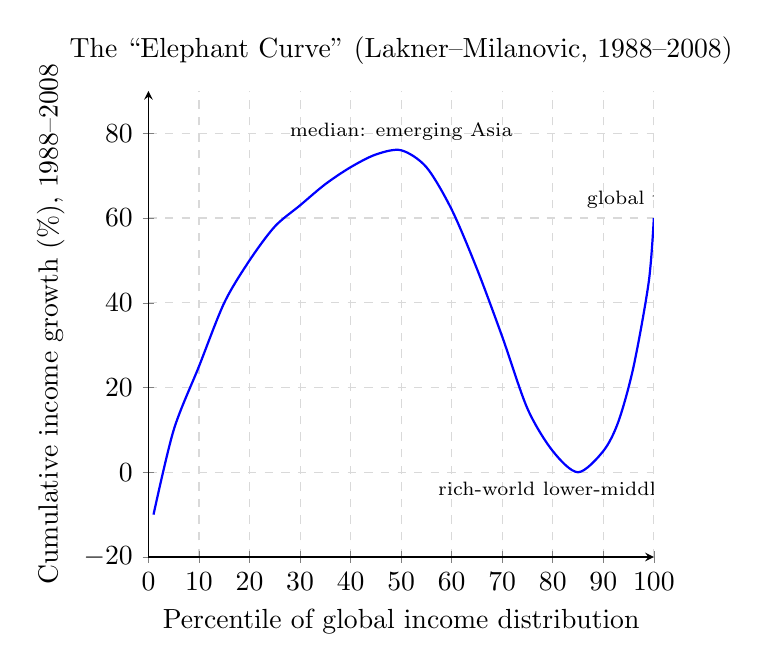
\begin{tikzpicture}
\begin{axis}[
    width=8cm, height=7.5cm,
    xlabel={Percentile of global income distribution},
    ylabel={Cumulative income growth (\%), 1988--2008},
    xmin=0, xmax=100,
    ymin=-20, ymax=90,
    xtick={0,10,20,30,40,50,60,70,80,90,100},
    ytick={-20,0,20,40,60,80},
    grid=major,
    grid style={dashed, gray!30},
    axis lines=left,
    title={The ``Elephant Curve'' (Lakner--Milanovic, 1988--2008)},
]
\addplot[thick, color=blue, mark=none, smooth] coordinates {
    (1,   -10)
    (5,    10)
    (10,   25)
    (15,   40)
    (20,   50)
    (25,   58)
    (30,   63)
    (35,   68)
    (40,   72)
    (45,   75)
    (50,   76)
    (55,   72)
    (60,   62)
    (65,   48)
    (70,   32)
    (75,   15)
    (80,    5)
    (85,    0)
    (90,    5)
    (93,   12)
    (96,   25)
    (99,   45)
    (100,  60)
};
\node[above] at (axis cs:50,76) {\scriptsize median: emerging Asia};
\node[below] at (axis cs:85,0) {\scriptsize rich-world lower-middle class};
\node[above] at (axis cs:100,60) {\scriptsize global top 1\%};
\end{axis}
\end{tikzpicture}
\end{document}